\cia\vspace{-2cm}
\section{Radiative correction}
The $\pi^0$ production illustrated in \F{fig:rad} a) is not the only process 
contributing to the electroproduction cross section. A photon or a $e^+e^- $ pair could be produced as well
and the amplitudes of these processes interfere with each other.
The measured $W, Q^2$  changes in case of radiation (for 
example the momentum of a scattered electron that emits a photon differs from the one at the 
leptonic vertex of \F{fig:rad} b) so a {\em radiative correction} is necessary. 


The  following radiative processes are present (in the lowest order of the fine structure constant).
\begin{itemize}
\item
the Bremsstrahlung, \F{fig:rad} b) and c) where a photon is emitted by the incoming or outgoing electron.
\item
the vertex correction, \F{fig:rad} d), where a photon is emitted by the incoming electron and 
absorbed by the outgoing
electron.
\item the vacuum polarization, \F{fig:rad} e), 
where the virtual photon produces temporarily an $e^+e^-$ pair.
\end{itemize}

\begin{figure}[h]
 \begin{center}
  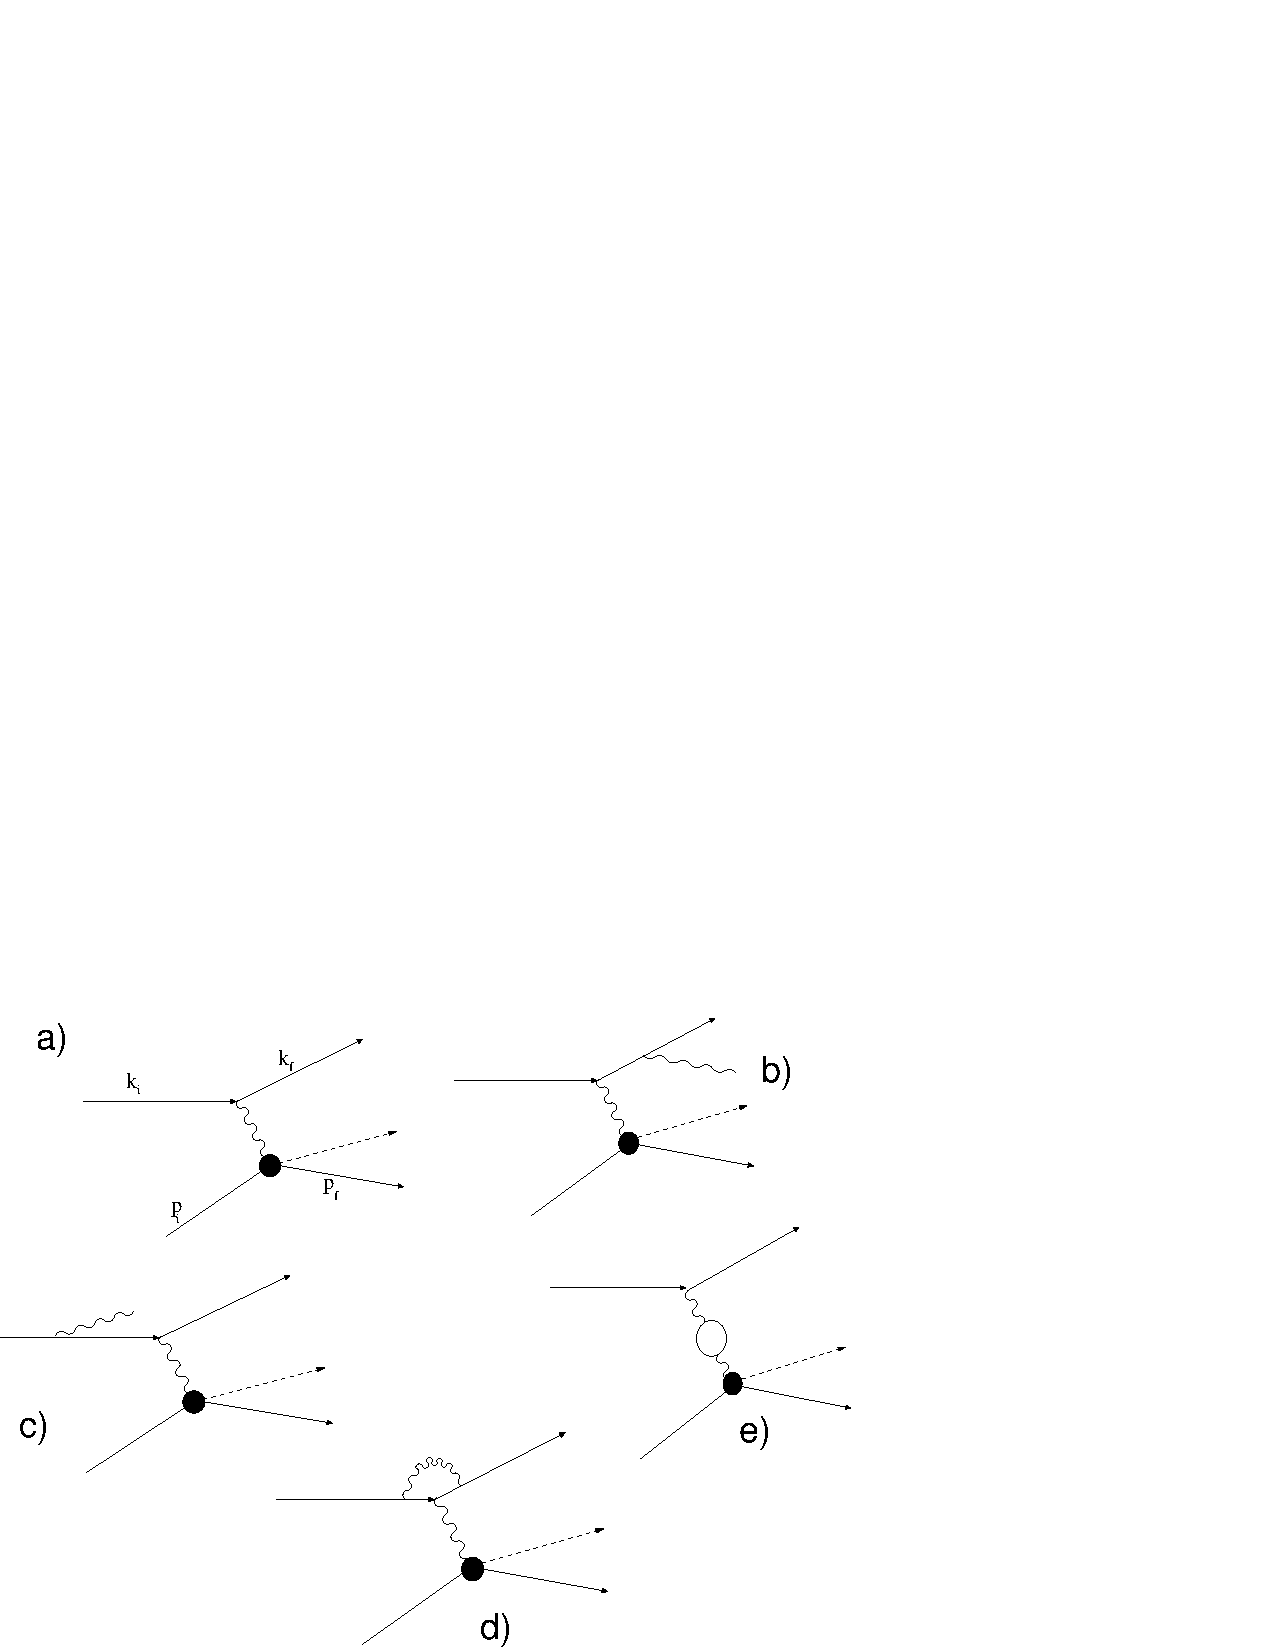
\includegraphics[width=14cm, bb=-60 -40 480 380]{analysis/img/rad}
  \caption[Feynman diagrams for the Born and radiative processes]
          { Feynman diagrams for the Born and radiative processes.
	             a) Born electroproduction, b) and c) Bremsstrahlung d) vertex
		     correction, e) vacuum polarization.}
 \label{fig:rad}
  \end{center} 
\end{figure} 

To account for the radiative processes the approach of reference \cite{bib:radcorr}, which is based on a 
covariant method for infrared cancellation \cite{bib:radinfra}, is used . 
Multiple soft photon radiation is included via exponentiation \cite{bib:shum}, \cite{bib:YFS}.
This method is preferred
over Mo and Tsai the procedure \cite{bib:motsai} because:

\begin{itemize}
\item[1)] It addresses {\it exclusive}
electroproduction rather than inclusive, thus involving all four unpolarized structure functions, as opposed to
the Mo and Tsai formalism which accounts only for two structure functions and inclusive scattering and it is independent of
outgoing hadron angles.
In principle, the general formulas of Mo and Tsai can be adapted to the coincidence framework if the integration
over the photon phase space is done properly. 

\item[2)] The infrared cancellation is independent of the unphysical
parameter $\Delta$ separating the phase space of soft and hard photons 
necessary in the Mo and Tsai procedure and leading to uncertainties.

\item[3)] The approach of ref. \cite{bib:radcorr} does not rely on the peaking approximation, avoiding
uncertainties at a few percent level associated with it.

\end{itemize}

The matrix element of the unradiated process \F{fig:rad} a) can be written as
\begin{equation}
 M^2 = \Dfrac{e^4}{Q^4}L_{\mu\nu}W^{\mu\nu}
 \label{eqno:mzero}
\end{equation}
where $L_{\mu\nu}$ and $W^{\mu\nu}$ are the leptonic and hadronic tensors:
\begin{equation}
L_{\mu\nu} = \Dfrac{1}{2}\,Tr\,(\slashed{k}_f+m)\gamma_\mu(\slashed{k}_i+m)(1+{\it i}\gamma_5\xi)\gamma_\nu 
\label{eqno:lepttens}
\end{equation}

The leptonic tensor for the radiative processes illustrated in \F{fig:rad} b), c), d) and e) changes into
\begin{equation}
L_{\mu\nu}^R = \Dfrac{1}{2}\,Tr\,(k_f+m)\Gamma_{\mu\alpha}(k_i+m)(1+{\it i}\gamma_5\xi)\hat{\Gamma}_{\alpha\nu}
\end{equation}
where the tensor $\Gamma_{\mu\alpha}$ contains the photon information $k^\mu_\gamma$.

The contraction of $L_{\mu\nu}^R$ with  $W^{\mu\nu}$ gives the matrix element $ M^2_R $ for the radiative processes:

\begin{equation}
 M^2_R = -\Dfrac{2e^6}{\tilde{Q}^4}L_{\mu\nu}^RW^{\mu\nu} =  -\Dfrac{2e^6}{\tilde{Q}^4R_w} \sum_{i=1}^{5}\theta_i H_i
 \label{eqno:radcorr}
\end{equation}
where $\tilde{Q^2} = -(q-k_\gamma)^2$ and $R_w = W^2 - (p+q-k_\gamma)^2$. One can see the involvement of all 
the structure functions $H_i$ and the intuitive modification to the normal definitions of $\tilde{Q^2}$ and $R_w$
with the presence of a radiated photon.

\begin{figure}[h]
 \begin{center}
  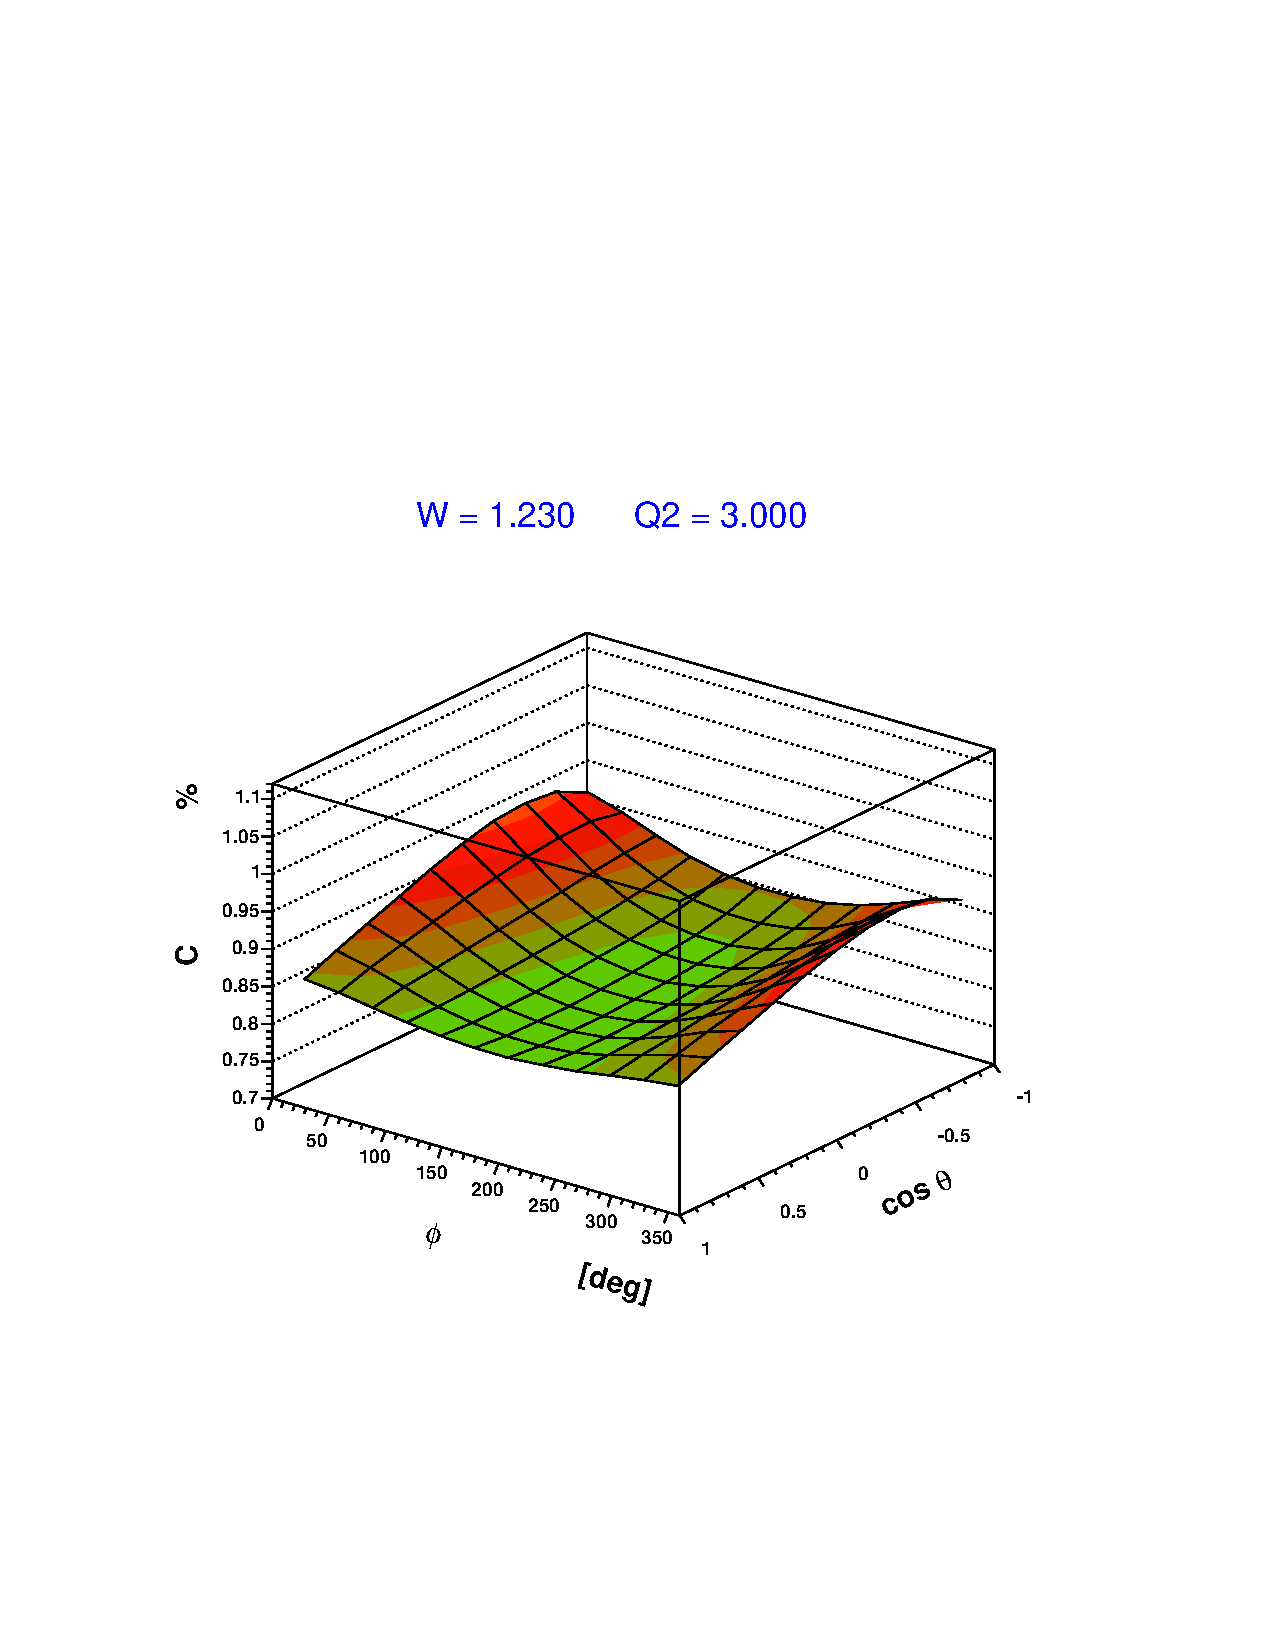
\includegraphics[width=15cm, bb=0 130 540 600]{analysis/img/costheta_phi_radcor_w1.23_q3.00}
  \caption[Radiative correction as a function of $\cos\theta^*$ and $\phi^*$ for $W=1.23$ GeV and $Q^2=3$ GeV$^2$]
          { Radiative correction as a function of $\cos\theta^*$ and $\phi^*$ for $W=1.23$ GeV and $Q^2=3$ GeV$^2$.}
 \label{fig:costheta_phi_radcor_w1.23_q3.00}
  \end{center} 
\end{figure} 

A program named {\it EXCLURAD} which is described in \cite{bib:radcorr} has been developed to calculate the matrix element (\ref{eqno:radcorr}) using
existing models (like MAID or DMT) for the structure functions. This program gives the radiative correction C as the ratio of the radiative
and unradiative four fold cross section:
$$
C(W, Q^2, \cos\theta^*, \phi^*) =\Dfrac{\sigma_{RAD}}{\sigma_{UNRAD}}
$$
which has been used as the radiative correction in this analysis.
Dependance on the missing mass cutoff parameter is tacit.
\F{fig:costheta_phi_radcor_w1.23_q3.00} shows the correction as a function 
of $\cos\theta^*$ and $\phi^*$ for $W=1.23$ GeV and $Q^2=3$ GeV$^2$.
Note that this procedure is different from that one followed for our published lower $Q^2$ data.
See    \begin{verbatim} 
http://www.jlab.org/~ungaro/pi0eprod/rad_plots/
\end{verbatim}
for the correction in each bin considered as a function of $\phi^*$ or $\cos\theta^*$.































